% ============================================================
% STRIDE Analysis — Milestone 1
% Network Security Lab Project — ULB 2026
% ============================================================
\documentclass[a4paper,12pt]{article}

\usepackage[utf8]{inputenc}
\usepackage[T1]{fontenc}
\usepackage[english]{babel}
\usepackage[margin=2.5cm]{geometry}
\usepackage{parskip}
\usepackage{microtype}
\usepackage{graphicx}
\usepackage{float}
\usepackage{lmodern}
\usepackage[dvipsnames,table]{xcolor}
\usepackage{booktabs}
\usepackage{tabularx}
\usepackage{array}
\usepackage{tikz}
\usetikzlibrary{matrix, positioning, fit, backgrounds}
\usepackage[colorlinks=true, linkcolor=black, urlcolor=blue]{hyperref}
\usepackage{fancyhdr}

% --- Couleurs heatmap ---
\definecolor{veryLowGreen}{HTML}{5CB85C}
\definecolor{lowGreen}    {HTML}{82C882}
\definecolor{modYellow}   {HTML}{F0C040}
\definecolor{highPink}    {HTML}{E05080}
\definecolor{critRed}     {HTML}{C0392B}

% --- Couleurs légende scoring ---
\definecolor{riskLow}    {HTML}{C8E6C9}
\definecolor{riskMedium} {HTML}{FFF9C4}
\definecolor{riskHigh}   {HTML}{FFCC80}
\definecolor{riskCrit}   {HTML}{FFCDD2}

% --- En-tête / pied de page ---
\pagestyle{fancy}
\fancyhf{}
\lhead{\small INFO-H303 : Network security}
\rhead{\small STRIDE Analysis --- Milestone 1}
\cfoot{\thepage}

% --- Macro cellule heatmap ---
\newlength{\CW}\setlength{\CW}{2.6cm}
\newlength{\CH}\setlength{\CH}{1.5cm}
\newcommand{\hcell}[4]{%
  \node[rectangle, rounded corners=6pt, fill=#1, text=white,
    minimum width=\CW, minimum height=\CH,
    font=\footnotesize\bfseries, align=center, inner sep=4pt]
  at (#3*2.75cm, #4*1.75cm) {#2};%
}

% ============================================================
\begin{document}
% ============================================================

% --- Page de titre ---
\begin{titlepage}
  \centering
  \vspace*{2cm}
  {\LARGE\textbf{Network Security --- Lab Project}}\\[0.5em]
  {\large Université Libre de Bruxelles}\\[2em]
  \rule{\linewidth}{0.4pt}\\[0.8em]
  {\huge\textbf{STRIDE Threat Analysis}}\\[0.4em]
  {\Large Milestone 1 --- Initial Setup}\\[0.4em]
  \rule{\linewidth}{0.4pt}\\[2em]
  {\large March 2026}\\[1em]
  {\normalsize Teaching Assistant: Navid Ladner
    (\texttt{navid.ladner@ulb.be})}\\[2em]
  \begin{tabular}{ll}
    Fernandez Ojeda Franklin   & (000541971) \\[0.4em]
    Lecky-Thompson William     & (000613648) \\[0.4em]
    Otto Aleksandra            & (000569128) \\[0.4em]
    Rafaat Moheeb Eskandar Abanoub & (000567614) \\
  \end{tabular}
  \vfill
\end{titlepage}

% ============================================================
\section*{Introduction}
\addcontentsline{toc}{section}{Introduction}
% ============================================================

Modern enterprise networks are exposed to a wide range of security threats, including external attacks, insider misuse, and protocol vulnerabilities. To address these risks, security engineering relies on threat modelling, a process used to identify, classify, and prioritise potential attacks before they occur.

In this project, we consider a simplified enterprise network composed of an Internet zone, an office network, and a server network hosting web services. At this stage, the infrastructure is not protected by any VPN or firewall, making it particularly exposed to various threats.

To analyse these risks, we use the STRIDE methodology, a framework that categorises threats into six types: Spoofing, Tampering, Repudiation, Information Disclosure, Denial of Service, and Elevation of Privilege.

% ============================================================
\section{Network Topology}
% ============================================================

The initial topology consists of three distinct network segments,
connected in a chain through routers configured with RIPv2:

\begin{itemize}
  \item External zone (Internet): Remote-Employee,
        Malicious~PC, Router~R1
  \item Office network: PC-1 (IT Dept.), PC-2 (HR Dept.),
        Router~R2
  \item Server network: Server-1 and Server-2 (NGINX),
        Router~R3
\end{itemize}

% ============================================================
\section{Identified Data Flows}
% ============================================================

The table below lists the seven data flows identified in the initial
topology, along with the applicable STRIDE threat categories for each.

\begin{center}
\begin{tabularx}{\textwidth}{cXl}
  \toprule
  \textbf{Flow} & \textbf{Description} & \textbf{STRIDE threats} \\
  \midrule
  F1 & Remote-Employee $\to$ R1 $\to$ R2 $\to$ PC-1/PC-2
     & S, I, T, E \\
  F2 & Malicious~PC $\to$ R1 $\to$ R2 $\to$ PC-1/PC-2
     & S, E, D, I, T \\
  F3 & PC-1/PC-2 $\to$ R2 $\to$ R3 $\to$ Servers
     & I, T, R \\
  F4 & Malicious~PC $\to$ R1 $\to$ R2 $\to$ R3 $\to$ Servers
     & E, D, T, I \\
  F5 & Server $\to$ R3 $\to$ R2 $\to$ PC-1/PC-2
     & E, T, D \\
  F6 & RIPv2: R1 $\leftrightarrow$ R2 $\leftrightarrow$ R3
     & S, T, D \\
  F7 & HTTP responses from NGINX servers
     & I, R, T \\
  \bottomrule
\end{tabularx}
\end{center}

\begin{figure}[H]
    \centering
    
\includegraphics[width=1\linewidth]{Network Security//Lab//img/STRIDE6.png}
    \label{fig:placeholder}
\end{figure}
% ============================================================
\section{Selected Attacks}
% ============================================================

From the STRIDE analysis of the network flows, five representative
attacks were selected based on their feasibility and potential impact.

% ------------------------------------------------------------
\subsection{A1 : Unauthorised access to servers (Elevation of Privilege)}
% ------------------------------------------------------------

For this attack, the attacker exploits the absence of filtering
mechanisms to gain unauthorised access to internal servers. The attack
uses flow F4, which allows a Malicious PC to reach Server-1 and
Server-2 through the path R1 $\to$ R2 $\to$ R3. Since no firewall or
access control is in place, this communication is not restricted. An
attacker could therefore exploit a vulnerability in the NGINX service
to compromise one of the servers. The risk score for this attack is
Likelihood 4 and Impact 5, resulting in a score of \textbf{20 (Critical)}.

To mitigate this attack, a firewall should be deployed between the
office network and the server network. Only authorised traffic,
specifically from PC-1 (IT Department), should be allowed to reach the
servers. In addition, access control lists (ACLs) should be configured
on R3 to enforce strict filtering policies.

% ------------------------------------------------------------
\subsection{A2 : IP Spoofing of the Remote-Employee (Spoofing)}
% ------------------------------------------------------------

For this attack, the attacker impersonates a legitimate remote employee
by forging their IP address. The attack relies on flows F1 and F2,
which allow communication between the external network and the office
network without authentication. In the absence of a VPN or identity
verification mechanism, the network cannot distinguish between a
legitimate user and a malicious actor. The risk score is Likelihood 4
and Impact 4, giving a total of \textbf{16 (High)}.

To mitigate this attack, a VPN with mutual certificate-based
authentication should be implemented. This ensures that only legitimate
users possessing valid certificates can establish a secure and trusted
connection to the internal network.

% ------------------------------------------------------------
\subsection{A3 : RIPv2 Route Poisoning (Tampering)}
% ------------------------------------------------------------

For this attack, an internal or already-compromised attacker manipulates
routing information to redirect network traffic. The attack uses flow F6,
which corresponds to routing updates exchanged via RIPv2 between R1, R2,
and R3. Since no authentication is enabled in the initial configuration,
any host present on one of the internal network segments (whether a
malicious insider, a compromised workstation, or a machine that has
already gained a foothold through a prior attack such as A1) can inject
forged routing announcements. This leads to route poisoning and can
enable man-in-the-middle attacks across the network, silently intercepting
or altering traffic between the office and server zones. The risk score
is Likelihood 3 and Impact 5, resulting in \textbf{15 (High)}.

To mitigate this attack, authentication mechanisms such as MD5 should
be enabled for RIPv2. Additionally, route filtering using
\texttt{distribute-list} should be configured to ensure that only
expected and trusted routes are accepted.

% ------------------------------------------------------------
\subsection{A4 : SYN/HTTP Flood against NGINX (Denial of Service)}
% ------------------------------------------------------------

For this attack, the attacker aims to disrupt service availability by
overloading the web servers. The attack targets flows F4 and F7, which
expose the NGINX servers to external traffic. Without any rate limiting
or protection mechanisms, an attacker can launch SYN or HTTP flooding
attacks to exhaust server resources and deny access to legitimate users.
The risk score is Likelihood 4 and Impact 3, resulting in
\textbf{12 (Elevated)}.

To mitigate this attack, rate limiting should be configured on the
NGINX servers using mechanisms such as \texttt{limit\_req\_zone}.
SYN cookies should also be enabled at the operating system level to
protect against SYN floods. Furthermore, access restrictions can be
enforced through ACLs on R3.

% ------------------------------------------------------------
\subsection{A5 : Lateral Movement from a Compromised Server (Elevation of Privilege)}
% ------------------------------------------------------------

For this attack, the attacker leverages a previously compromised server
to move laterally within the network. The attack uses flow F5, which
allows communication from the server network to the office network.
Once a server is compromised, nothing prevents it from initiating
connections toward internal workstations, potentially leading to
further compromise and data exfiltration. The risk score is Likelihood 3
and Impact 5, resulting in \textbf{15 (High)}.

To mitigate this attack, strict network segmentation must be enforced.
Firewall rules should explicitly block any traffic initiated from the
server network toward the office network. This ensures adherence to the
principle of least privilege and limits the potential impact of a
compromise.
% ============================================================
\section{Risk Heatmap}
% ============================================================

The heatmap below places each of the five attacks on a
$5 \times 5$ Likelihood~$\times$~Impact grid. The colour of each
cell indicates the risk level.

\begin{center}
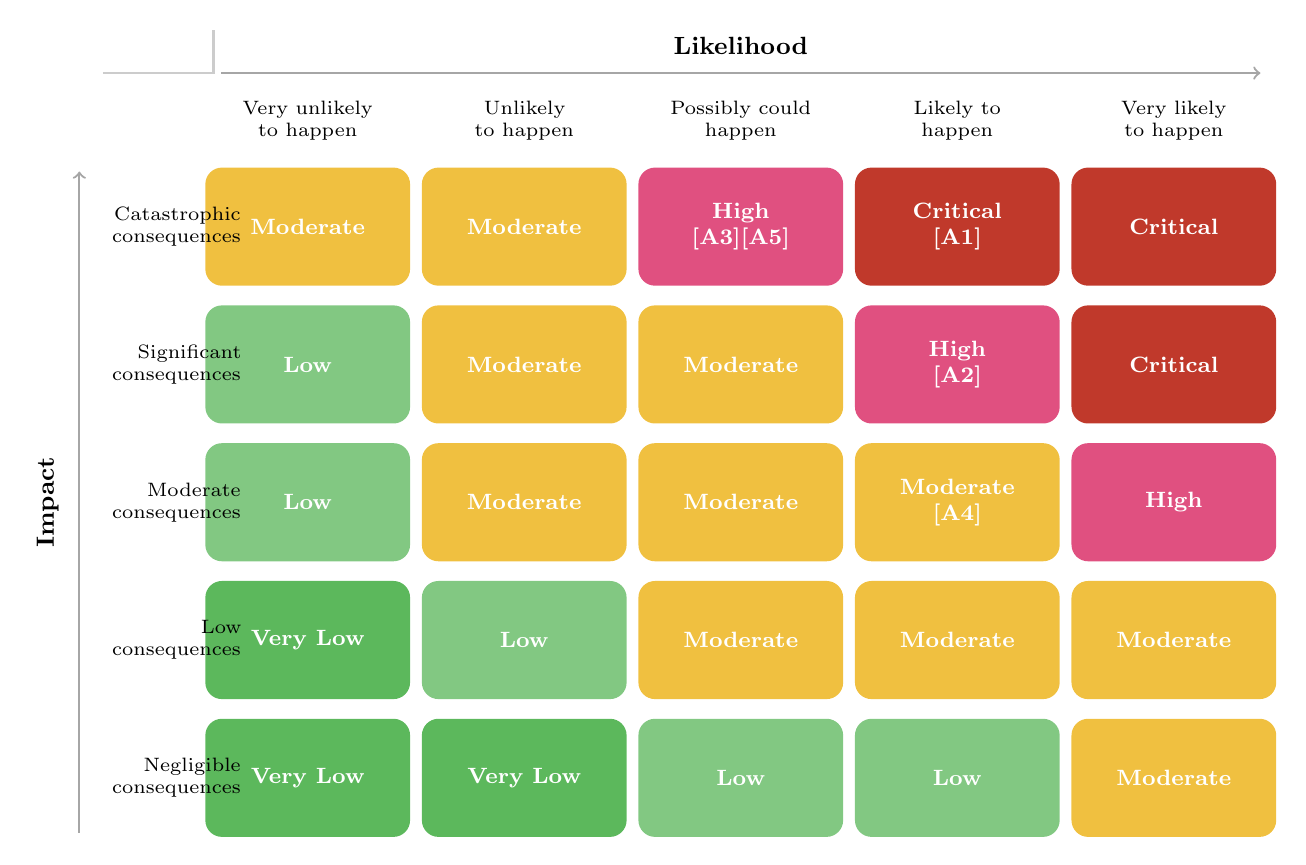
\begin{tikzpicture}

% --- CELLS ---
% ROW 4 : Catastrophic
\hcell{modYellow}{Moderate}           {0}{4}
\hcell{modYellow}{Moderate}           {1}{4}
\hcell{highPink} {High\\{[A3][A5]}}   {2}{4}
\hcell{critRed}  {Critical\\{[A1]}}   {3}{4}
\hcell{critRed}  {Critical}           {4}{4}
% ROW 3 : Significant
\hcell{lowGreen} {Low}                {0}{3}
\hcell{modYellow}{Moderate}           {1}{3}
\hcell{modYellow}{Moderate}           {2}{3}
\hcell{highPink} {High\\{[A2]}}       {3}{3}
\hcell{critRed}  {Critical}           {4}{3}
% ROW 2 : Moderate
\hcell{lowGreen} {Low}                {0}{2}
\hcell{modYellow}{Moderate}           {1}{2}
\hcell{modYellow}{Moderate}           {2}{2}
\hcell{modYellow}{Moderate\\{[A4]}}   {3}{2}
\hcell{highPink} {High}               {4}{2}
% ROW 1 : Low
\hcell{veryLowGreen}{Very Low}        {0}{1}
\hcell{lowGreen}    {Low}             {1}{1}
\hcell{modYellow}   {Moderate}        {2}{1}
\hcell{modYellow}   {Moderate}        {3}{1}
\hcell{modYellow}   {Moderate}        {4}{1}
% ROW 0 : Negligible
\hcell{veryLowGreen}{Very Low}        {0}{0}
\hcell{veryLowGreen}{Very Low}        {1}{0}
\hcell{lowGreen}    {Low}             {2}{0}
\hcell{lowGreen}    {Low}             {3}{0}
\hcell{modYellow}   {Moderate}        {4}{0}

% --- COLUMN HEADERS (Likelihood) ---
\foreach \col/\lbl in {
  0/{Very unlikely\\to happen},
  1/{Unlikely\\to happen},
  2/{Possibly could\\happen},
  3/{Likely to\\happen},
  4/{Very likely\\to happen}
}{
  \node[font=\scriptsize, align=center, text width=2.4cm]
    at (\col*2.75cm, 4*1.75cm + 1.35cm) {\lbl};
}
\node[font=\small\bfseries] at (2*2.75cm, 4*1.75cm + 2.3cm) {Likelihood};
\draw[->, thick, gray!70]
  (-1.1cm, 4*1.75cm + 1.95cm) -- (4*2.75cm + 1.1cm, 4*1.75cm + 1.95cm);

% --- ROW HEADERS (Impact) ---
\foreach \row/\lbl in {
  4/{Catastrophic\\consequences},
  3/{Significant\\consequences},
  2/{Moderate\\consequences},
  1/{Low\\consequences},
  0/{Negligible\\consequences}
}{
  \node[font=\scriptsize, align=right, text width=2.3cm]
    at (-2.0cm, \row*1.75cm) {\lbl};
}
\node[font=\small\bfseries, rotate=90] at (-3.3cm, 2*1.75cm) {Impact};
\draw[->, thick, gray!70]
  (-2.9cm, -0.7cm) -- (-2.9cm, 4*1.75cm + 0.7cm);

% Decorative corner line
\draw[gray!40, line width=1pt]
  (-2.6cm, 4*1.75cm + 1.95cm) -- (-1.2cm, 4*1.75cm + 1.95cm)
  -- (-1.2cm, 4*1.75cm + 2.5cm);

\end{tikzpicture}
\end{center}

\medskip
\noindent
The table below summarises the position of each attack on the grid:

\begin{center}
\begin{tabular}{clccc}
  \toprule
  \textbf{Attack} & \textbf{Threat type} & \textbf{Likelihood}
    & \textbf{Impact} & \textbf{Score} \\
  \midrule
  A1 & Elevation of Privilege & 4 & 5 & 20 --- Critical \\
  A2 & Spoofing               & 4 & 4 & 16 --- High     \\
  A3 & Tampering              & 3 & 5 & 15 --- High     \\
  A4 & Denial of Service      & 4 & 3 & 12 --- Elevated \\
  A5 & Elevation of Privilege & 3 & 5 & 15 --- High     \\
  \bottomrule
\end{tabular}
\end{center}

\medskip\noindent
\textbf{A1} (score 20) is the most critical attack: it is both easy
to carry out and potentially devastating, as it gives an attacker
direct control over a server. \textbf{A2} (score 16) ranks just
below, in the High zone : it does not reach the Critical level
because compromising the office PCs, while serious, has a lower
impact than full server compromise. \textbf{A3} and \textbf{A5}
(both score 15, High) require a precondition : being present on the
internal network or having already compromised a host for A3, or
having already compromised a server for A5, which lowers their
likelihood. \textbf{A4} (score 12, Elevated) is easy to
execute but has a limited impact since the servers do not hold
critical data in this initial setup.

% ============================================================
\section{Summary}
% ============================================================

The table below maps each identified attack to the security component
that addresses it in Milestone~1.

\begin{center}
\begin{tabularx}{\textwidth}{cXXc}
  \toprule
  \textbf{Attack} & \textbf{Main threat} & \textbf{Mitigation}
  & \textbf{Score} \\
  \midrule
  A1 & Unauthorised server access (E)
     & Firewall: block external traffic towards R3 & 20 \\
  A2 & IP Spoofing (S)
     & Site-to-site VPN with certificates & 16 \\
  A3 & RIPv2 route poisoning (T)
     & MD5 auth on RIPv2 + distribute-list & 15 \\
  A4 & SYN/HTTP flood NGINX (D)
     & ACLs on R3 + NGINX rate limiting & 12 \\
  A5 & Server pivot to office (E)
     & Firewall: block server-initiated traffic & 15 \\
  \bottomrule
\end{tabularx}
\end{center}

Attacks A1 and A2 are the most critical and directly motivate the
two security components required in Milestone~1: the \textbf{Firewall}
and the \textbf{VPN}. A3 and A5, while also serious, will be partially
addressed as a side effect of the firewall deployment. A4 will be
more fully mitigated in Milestone~2 with the Web Application Firewall.

\end{document}